% !TeX encoding = UTF-8
% !TeX program = xelatex
% !TeX spellcheck = en_US

\documentclass[degree=master,language=english,cjk-font=external]{sustechthesis}
  % 学位 degree:
  %   master (默认) | doctor
  % 语言 language:
  %   chinese (默认)| english
  % 中文字体 cjk-font
  %   auto (默认,自动选择系统自带字体)| external (包内字体)| windows | mac | 等
  %   在 **非Windows** 的系统上推荐使用包内字体,而非系统字体。
  %   以达到和 Windows 系统上显示的字体效果。
  %   Windows 系统上可以删除该参数,使用系统内置字体。


% 论文基本配置,加载宏包等全局配置
% !TeX root = ./sustechthesis-example.tex

% 论文基本信息配置

\thusetup{
  %******************************
  % 注意:
  %   1. 配置里面不要出现**空行**
  %   2. 不需要的配置信息可以删除
  %   3. 建议先阅读文档中所有关于选项的说明
  %******************************
  %
  % 输出格式
  %   选择打印版(print)或用于提交的电子版(electronic),前者会插入空白页以便直接双面打印
  %
  output = electronic,
  %
  % 标题
  %   可使用“\\”命令手动控制换行
  %   如果需要使用副标题,取消 subtitle 和 subtitle* 的注释即可。
  %
  title  = {南方科技大学学位论文 \LaTeX{} 模板 (Support English) 使用示例文档 v\version},
  title* = {An Introduction to \LaTeX{} Thesis Template of Southern University of Science and Technology v\version},
  % subtitle = {可选的副标题可选的副标题可选的副标题可选的副标题可选的副标题可选的副标题},
  % subtitle* = {optional subtitle optional subtitle optional subtitle optional subtitle optional subtitle optional subtitle},
  %
  % 学位
  %
  degree-domain = {工学}, % 【中文】学科门类:可选理学、工学、医学
  degree-domain* = {Engineering}, % 【英文】学位等级:可选Science, Engineering, Medicine
  gongshuo = false, % 是否为专业型学位。专业型学位则填 true ,学术型或其他为 false 。
  %
  % 培养单位
  %   填写所属院系的全名
  %   超长英文系名可以手动换行
  department = {计算机科学与工程系},
  department* = {School of System Design and \\Intelligent Manufacturing},
  %
  % 学科
  %   1. 学术型学位
  %      获得一级学科授权的学科填写一级学科名称,其他填写二级学科名称
  %   2. 工程硕士
  %      工程领域名称
  %
  discipline  = {计算机科学与技术},
  discipline* = {Computer Science and Technology},
  %
  % 姓名
  %   英文用全拼,姓在前,名在后,姓和名的首字母大写,其余小写
  %
  author  = {李子强},
  author* = {Li Ziqiang},
  %
  % 指导教师
  %   中文姓名和职称之间以英文逗号“,”分开,下同
  %
  supervisor  = {某某某(Alice Bob)助理教授},
  supervisor* = {Assistant Professor Alice Bob},
  %
  % 日期
  %   使用 ISO 格式;默认为当前时间
  %   date 为第一页全中文大写日期,defense-date 为第二、三页的答辩日期。
  %   需要按 {年-月-日} 格式填写,如不显示“日”,可以随意填一个日期,但是不能为空。
  %
  date = {2020-12-20},
  defense-date = {2020-12-20},
  %
  % 密级
  %   公开, 秘密, 机密, 绝密
  %
  statesecrets={公开},
  %
  % 国内图书分类号,国际图书分类号
  %
  natclassifiedindex={TM301.2},
  intclassifiedindex={62-5},
}

% 载入所需的宏包

% 可以使用 nomencl 生成符号和缩略语说明
% \usepackage{nomencl}
% \makenomenclature

% 表格加脚注
\usepackage{threeparttable}

% 表格中支持跨行
\usepackage{multirow}

% 量和单位
\usepackage{siunitx}

% 定理类环境宏包
\usepackage{amsthm}
% 也可以使用 ntheorem
% \usepackage[amsmath,thmmarks,hyperref]{ntheorem}

%%%%%% 参考文献编译方式二选一,不要同时开启。
%%%% 选择一
%% 参考文献使用 BibTeX + natbib 宏包
%% 顺序编码制
\usepackage[sort&compress]{gbt7714}
\bibliographystyle{gbt7714-numerical}
\usepackage{bibunits}

%%%% 选择二(不兼容本模板,请勿使用)
%% 参考文献使用 BibLaTeX 宏包
% \usepackage[backend=biber,style=gb7714-2015]{biblatex}
%% 声明 BibLaTeX 的数据库
% \addbibresource{ref/refs.bib}

% 定义所有的图片文件在 figures 子目录下
\graphicspath{{figures/}}

% 数学命令
\newcommand\dif{\mathop{}\!\mathrm{d}}  % 微分符号

% hyperref 宏包在最后调用
\usepackage{hyperref}
\usepackage{ragged2e}

% 固定宽度的表格。放在 hyperref 之前的话,tabularx 里的 footnote 显示不出来。
\usepackage{tabularx}

% 跨页表格,必须在 hyperref 之后使用否则会报错。
\usepackage{longtable}



\begin{document}

% 封面
\maketitle

% 学位论文公开评阅人和答辩委员会名单
% !TeX root = ../sustechthesis-example.tex




% 南方科技大学学位论文原创性声明和使用授权说明
% 本模版不会对扫描版的页码进行处理,建议定稿后打印声明页再插入编译,以免页码出错。
% 或者,使用其他 pdf 拼接软件也可达到替换声明页面的目的。
\statementcopyright % 生成未签名的声明
% \statementcopyright[scan-statement.pdf] % 插入已签名的声明文件(扫描版)

\frontmatter
% !TeX root = ../sustechthesis-example.tex

% 中英文摘要和关键字

\begin{abstract}
  论文的摘要是对论文研究内容和成果的高度概括。
  摘要应对论文所研究的问题及其研究目的进行描述,对研究方法和过程进行简单介绍,对研究成果和所得结论进行概括。
  摘要应具有独立性和自明性,其内容应包含与论文全文同等量的主要信息。
  使读者即使不阅读全文,通过摘要就能了解论文的总体内容和主要成果。

  论文摘要的书写应力求精确、简明。
  切忌写成对论文书写内容进行提要的形式,尤其要避免“第 1 章……;第 2 章……;……”这种或类似的陈述方式。
  
  博士论文摘要约 800~1000 字,硕士论文摘要的字数一般为 500 字左右,且篇幅限制在一页内书写。

  关键词是为了文献标引工作、用以表示全文主要内容信息的单词或术语。
  关键词不超过 5 个,每个关键词中间用分号分隔。

  % 关键词用“英文逗号”分隔,输出时会自动处理为正确的分隔符
  \thusetup{
    keywords = {关键词 1, 关键词 2, 关键词 3, 关键词 4, 长长长长长长长长长长长长长长长长长长长长长长长长长关键词 5},
  }
\end{abstract}

\begin{abstract*}
  An abstract of a dissertation is a summary and extraction of research work and contributions.
  Included in an abstract should be description of research topic and research objective, brief introduction to methodology and research process, and summarization of conclusion and contributions of the research.
  An abstract should be characterized by independence and clarity and carry identical information with the dissertation.
  It should be such that the general idea and major contributions of the dissertation are conveyed without reading the dissertation.

  An abstract should be concise and to the point.
  It is a misunderstanding to make an abstract an outline of the dissertation and words “the first chapter”, “the second chapter” and the like should be avoided in the abstract.

  The abstract of the doctoral thesis is about 800 to 1000 words; the abstract of the master's thesis is generally about 500 words; the length is limited to one page.

  Keywords are terms used in a dissertation for indexing, reflecting core information of the dissertation.
  An abstract may contain a maximum of 5 keywords, with semi-colons used in between to separate one another.

  % Use comma as seperator when inputting
  \thusetup{
    keywords* = {keyword 1, keyword 2, keyword 3, keyword 4, looooooooooooooooooooong keyword 5},
  }
\end{abstract*}


% 目录
\tableofcontents

% 插图和附表清单
% \listoffiguresandtables  % 插图和附表清单
% \listoffigures           % 插图清单
% \listoftables            % 附表清单

% 符号对照表(非强制性要求,如果论文中所用符号不多,可以略去)
% !TeX root = ../sustechthesis-example.tex

% denotation 环境带一个可选参数,用来指定符号列的宽度(默认为 2.5cm),下面改3cm为例。
\begin{denotation}[3cm]
  \item[PI] 聚酰亚胺
  \item[MPI] 聚酰亚胺模型化合物,N-苯基邻苯酰亚胺
  \item[PBI] 聚苯并咪唑
  \item[MPBI] 聚苯并咪唑模型化合物,N-苯基苯并咪唑
  \item[PY] 聚吡咙
  \item[PMDA-BDA] 均苯四酸二酐与联苯四胺合成的聚吡咙薄膜
  \item[MPY] 聚吡咙模型化合物
  \item[As-PPT] 聚苯基不对称三嗪
  \item[MAsPPT] 聚苯基不对称三嗪单模型化合物,3,5,6-三苯基-1,2,4-三嗪
  \item[DMAsPPT] 聚苯基不对称三嗪双模型化合物(水解实验模型化合物)
  \item[S-PPT] 聚苯基对称三嗪
  \item[MSPPT] 聚苯基对称三嗪模型化合物,2,4,6-三苯基-1,3,5-三嗪
  \item[PPQ] 聚苯基喹噁啉
  \item[MPPQ] 聚苯基喹噁啉模型化合物,3,4-二苯基苯并二嗪
  \item[HMPI] 聚酰亚胺模型化合物的质子化产物
  \item[HMPY] 聚吡咙模型化合物的质子化产物
  \item[HMPBI] 聚苯并咪唑模型化合物的质子化产物
  \item[HMAsPPT] 聚苯基不对称三嗪模型化合物的质子化产物
  \item[HMSPPT] 聚苯基对称三嗪模型化合物的质子化产物
  \item[HMPPQ] 聚苯基喹噁啉模型化合物的质子化产物
  \item[PDT] 热分解温度
  \item[HPLC] 高效液相色谱 (High Performance Liquid Chromatography)
  \item[HPCE] 高效毛细管电泳色谱 (High Performance Capillary lectrophoresis)
  \item[LC-MS] 液相色谱-质谱联用 (Liquid chromatography-Mass Spectrum)
  \item[TIC] 总离子浓度 (Total Ion Content)
  \item[\textit{ab initio}] 基于第一原理的量子化学计算方法,常称从头算法
  \item[DFT] 密度泛函理论 (Density Functional Theory)
  \item[$E_a$] 化学反应的活化能 (Activation Energy)
  \item[ZPE] 零点振动能 (Zero Vibration Energy)
  \item[PES] 势能面 (Potential Energy Surface)
  \item[TS] 过渡态 (Transition State)
  \item[TST] 过渡态理论 (Transition State Theory)
  \item[$\increment G^\neq$] 活化自由能(Activation Free Energy)
  \item[$\kappa$] 传输系数 (Transmission Coefficient)
  \item[IRC] 内禀反应坐标 (Intrinsic Reaction Coordinates)
  \item[$\nu_i$] 虚频 (Imaginary Frequency)
  \item[ONIOM] 分层算法 (Our own N-layered Integrated molecular Orbital and molecular Mechanics)
  \item[SCF] 自洽场 (Self-Consistent Field)
  \item[SCRF] 自洽反应场 (Self-Consistent Reaction Field)
\end{denotation}



% 也可以使用 nomencl 宏包,需要在导言区
% \usepackage{nomencl}
% \makenomenclature

% 在这里输出符号说明
% \printnomenclature[3cm]

% 在正文中的任意为都可以标题
% \nomenclature{PI}{聚酰亚胺}
% \nomenclature{MPI}{聚酰亚胺模型化合物,N-苯基邻苯酰亚胺}
% \nomenclature{PBI}{聚苯并咪唑}
% \nomenclature{MPBI}{聚苯并咪唑模型化合物,N-苯基苯并咪唑}
% \nomenclature{PY}{聚吡咙}
% \nomenclature{PMDA-BDA}{均苯四酸二酐与联苯四胺合成的聚吡咙薄膜}
% \nomenclature{MPY}{聚吡咙模型化合物}
% \nomenclature{As-PPT}{聚苯基不对称三嗪}
% \nomenclature{MAsPPT}{聚苯基不对称三嗪单模型化合物,3,5,6-三苯基-1,2,4-三嗪}
% \nomenclature{DMAsPPT}{聚苯基不对称三嗪双模型化合物(水解实验模型化合物)}
% \nomenclature{S-PPT}{聚苯基对称三嗪}
% \nomenclature{MSPPT}{聚苯基对称三嗪模型化合物,2,4,6-三苯基-1,3,5-三嗪}
% \nomenclature{PPQ}{聚苯基喹噁啉}
% \nomenclature{MPPQ}{聚苯基喹噁啉模型化合物,3,4-二苯基苯并二嗪}
% \nomenclature{HMPI}{聚酰亚胺模型化合物的质子化产物}
% \nomenclature{HMPY}{聚吡咙模型化合物的质子化产物}
% \nomenclature{HMPBI}{聚苯并咪唑模型化合物的质子化产物}
% \nomenclature{HMAsPPT}{聚苯基不对称三嗪模型化合物的质子化产物}
% \nomenclature{HMSPPT}{聚苯基对称三嗪模型化合物的质子化产物}
% \nomenclature{HMPPQ}{聚苯基喹噁啉模型化合物的质子化产物}
% \nomenclature{PDT}{热分解温度}
% \nomenclature{HPLC}{高效液相色谱 (High Performance Liquid Chromatography)}
% \nomenclature{HPCE}{高效毛细管电泳色谱 (High Performance Capillary lectrophoresis)}
% \nomenclature{LC-MS}{液相色谱-质谱联用 (Liquid chromatography-Mass Spectrum)}
% \nomenclature{TIC}{总离子浓度 (Total Ion Content)}
% \nomenclature{\textit{ab initio}}{基于第一原理的量子化学计算方法,常称从头算法}
% \nomenclature{DFT}{密度泛函理论 (Density Functional Theory)}
% \nomenclature{$E_a$}{化学反应的活化能 (Activation Energy)}
% \nomenclature{ZPE}{零点振动能 (Zero Vibration Energy)}
% \nomenclature{PES}{势能面 (Potential Energy Surface)}
% \nomenclature{TS}{过渡态 (Transition State)}
% \nomenclature{TST}{过渡态理论 (Transition State Theory)}
% \nomenclature{$\increment G^\neq$}{活化自由能(Activation Free Energy)}
% \nomenclature{$\kappa$}{传输系数 (Transmission Coefficient)}
% \nomenclature{IRC}{内禀反应坐标 (Intrinsic Reaction Coordinates)}
% \nomenclature{$\nu_i$}{虚频 (Imaginary Frequency)}
% \nomenclature{ONIOM}{分层算法 (Our own N-layered Integrated molecular Orbital and molecular Mechanics)}
% \nomenclature{SCF}{自洽场 (Self-Consistent Field)}
% \nomenclature{SCRF}{自洽反应场 (Self-Consistent Reaction Field)}



% 正文部分
\mainmatter
% !TeX root = ../sustechthesis-example.tex

\chapter{气体动理论}


\section{理想气体}


\section{速度分布函数与宏观量}\label{sec:Boltzmann}

在气体动理论中,单原子气体在相空间中的概率密度由速度分布函数$f(t,\bm{x},\bm{v})$表示,是时间$t$, 空间坐标$ \bm{x}=(x_1,x_2,x_3)$ 和 分子速度$\bm{v}=(v_1,v_2,v_3)$的函数. 定义$f(t,\bm{x},\bm{v})d\bm{x}d\bm{v}$是体积为$d\bm{x}d\bm{v}$的相空间上的分子数,则气体的数密度$n$、宏观速度$\bm{u}$、温度$T$、压力张量$p_{ij}$和热流$\bm{q}$可以分别通过对速度分布函数求矩得到:
\begin{equation}\label{macroscopic_origin}
\begin{aligned}[b]
&n(t,\bm{x})=\int{}f(t,\bm{x},\bm{v})d\bm{v}, \\  &\bm{u}(t,\bm{x})=\frac{1}{n(t,\bm{x})}\int\bm{v}f(t,\bm{x},\bm{v})d\bm{v},\\   &T(t,\bm{x})=\frac{m}{3k_Bn(t,\bm{x})}\int{}c^2f(t,\bm{x},\bm{v})d\bm{v}, \\    &p_{ij}(t,\bm{x})={}m\int{}c_ic_jf(t,\bm{x},\bm{v})d\bm{v}, \\  &\bm{q}(t,\bm{x})=\frac{m}{2}\int{}c^2\bm{c}f(t,\bm{x},\bm{v})d\bm{v},
\end{aligned}
\end{equation}
其中, $\bm{c}=\bm{v}-\bm{u}$是气体分子热运动速度, 即气体分子速度与当地宏观速度的矢量差,而$c$是热运动速率. 定义应力偏量为
\begin{equation}
\sigma_{ij}=p_{ij}-p\delta_{ij},
\end{equation}
其中$p=nk_BT$, $\delta_{ij}$为克罗内克函数. 


\section{Boltzmann方程}

The governing equation for the evolution of VDF of a dilute gas system is derived by Ludwig Boltzmann. In his description, molecules move in straight lines with fixed velocities until they encounter elastic collisions with other molecules. This is justified by the fact that, at standard temperature and pressure, the MFP of gas molecules is hundreds times of the nominal atomic diameter and about 30 times the average molecular separation.  

Both molecular streaming and collision change the VDF in the phase space as per the Boltzmann equation~\cite{CE,Cercignani1990,henning,Kremer2009book}:
\begin{equation}\label{Boltzmann}
\frac{\partial f}{\partial t}+\bm{v}\cdot\frac{\partial f}{\partial
	\bm{x}}+\bm{a}\cdot\frac{\partial f}{\partial \bm{v}}={Q(f,f_*)},
\end{equation}
where the first term on the left hand side describes the change of VDF with respect to time, the second term is the convective change, and the third term represents the change of VDF induced by external acceleration (suppose it is independent of the molecular velocity). They together describe the streaming of gas molecules. 

The quadratic collision operator $Q(f,f_*)$ describes the change of molecular numbers per unit phase-space volume $d\bm{x}d\bm{v}$ and per unit time. This change consists of two effects. First, when the molecule with velocity $\bm{v}$ collides with another molecule with velocity $\bm{v}_\ast$, its velocity becomes $\bm{v}'$, which contributes to the loss of  molecules with the very velocity $\bm{v}$. During time interval $\Delta{t}$, there are 
\begin{equation}\label{total_collision}
f(t,\bm{x},\bm{v}_\ast)v_r\Delta{t}bdbd\phi{}d\bm{v}_\ast
\end{equation}
such collisions. Therefore, the number of molecule lost in the binary collision per unit phase-space volume and per time is
\begin{equation}
\begin{aligned}[b]
Q_{\text{loss}}&=\frac{\int{}f(t,\bm{x},\bm{v})d\bm{x}d\bm{v}\times
	f(t,\bm{x},\bm{v}_\ast)v_r\Delta{t}bdbd\phi{}d\bm{v}_\ast}{d\bm{x}d\bm{v}\Delta{t}}\\
&=\frac{\int{}f(t,\bm{x},\bm{v})d\bm{x}d\bm{v}\times
	f(t,\bm{x},\bm{v}_\ast)v_r\Delta{t}
	\sigma_D\sin\theta{d\theta}d\phi{}d\bm{v}_\ast}{d\bm{x}d\bm{v}\Delta{t}}\\
&=\int_{\mathbb{R}^3}\int_{\mathbb{S}^{2}}
B(\cos\theta,v_r)
f(t,\bm{x},\bm{v}_{\ast})f(t,\bm{x},\bm{v})
d\Omega
d\bm{v}_\ast.
\end{aligned}
\end{equation}
Second, when the molecule with velocity $\bm{v}'$ collides with another molecule with the velocity $\bm{v}'_\ast$, its velocity becomes $\bm{v}$, which contributes to the gain of molecules with the very velocity $\bm{v}$. Therefore, with the facts that $d\bm{v}d\bm{v}_\ast=d\bm{v}'d\bm{v}'_\ast$, $v_r=v'_r$, and the collision kernel is only determined by the relative collision speed and impact parameter, the gain part of the Boltzmann collision operator is
\begin{equation}
\begin{aligned}[b]
Q_{\text{gain}}&=\frac{\int{}f(t,\bm{x},\bm{v}')d\bm{x}d\bm{v}'\times
	f(t,\bm{x},\bm{v}'_\ast)v'_r\Delta{t}bdbd\phi{}d\bm{v}'_\ast}{d\bm{x}d\bm{v}\Delta{t}}\\
&=\int_{\mathbb{R}^3}\int_{\mathbb{S}^{2}}
B(\cos\theta,v_r)
f(t,\bm{x},\bm{v}'_{\ast})f(t,\bm{x},\bm{v}')
d\Omega
d\bm{v}_\ast.
\end{aligned}
\end{equation}
Finally, the Boltzmann collision operator \index{Boltzmann collision operator} is written in the following form (since it is local in time and space, for simplicity $t$ and $\bm{x}$ will be omitted in writing the collision operator):
\begin{eqnarray}\label{chapter1_collision}
Q(f,f_*)=\int_{\mathbb{R}^3}\int_{\mathbb{S}^{2}}
B(\cos\theta,v_r)
[f(\bm{v}'_{\ast})f(\bm{v}')-
f(\bm{v}_{\ast})f(\bm{v})]
d\Omega
d\bm{v}_\ast.
\end{eqnarray}
Note that the ``Stosszahlansatz'' or assumption of molecular chaos was used implicitly, that is, the value of VDF for different velocities are independent. 

%

%The Boltzmann equation is more complicated than the NSF equations, not only because the VDF is defined in six-dimensional phase-space (three dimensional spatial space and three dimensional velocity space), but also because of its high dimensional collision operator (fivefold integral with three dimensions in velocity space and two dimensions in a unit sphere). Therefore, it is highly desirable to have macroscopic equations like the NSF ones. To eliminate the microscopic velocity variables, moment equations from the Boltzmann equation should be considered. Multiplying Eq.~\eqref{Boltzmann} by 1, $\bm{v}$, and $|\bm{v}|^2$, and integrating the resulting equations with respect to the molecular velocity $\bm{v}$, one gets Eqs.~\eqref{macro_denstiy}--\eqref{macro_temperature}. However, these equations are not closed because expressions for shear stress and heat flux are not known. 


对于稀疏气体 ~(dilute gas,分子间距远远大于分子直径),在外部施加的加速度$\bm{a}=(a_1,a_2,a_3)$的作用下,速度分布函数的演化由玻尔兹曼方程描述:
\begin{equation}\label{Boltzmann}
\frac{\partial f}{\partial t}+\bm{v}\cdot\frac{\partial f}{\partial
	\bm{x}}+\bm{a}\cdot\frac{\partial f}{\partial \bm{v}}={Q(f)}.
\end{equation}
方程左边的三项分别表示速度分布函数在时间上的变化,在速度作用下在物理空间的变化,以及在外力作用下在速度空间的变化;右边表示使得分布函数趋于平衡态的气体分子的碰撞过程. 在玻尔兹曼方程中,二体碰撞的形式为:
\begin{equation}\label{chapter1_collision}
Q(f)=\iint{}B(\theta,{v}_r) 
[f(\bm{v}'_*)f(\bm{v}')-f(\bm{v}_*)f(\bm{v})]d{\Omega}d\bm{v}_*.
\end{equation}
其中,$\bm{v}$ 和 $\bm{v}_\ast$ 分别是碰撞前两个分子的速度,而$\bm{v}'$ 和 $\bm{v}'_\ast$是它们碰撞后的速度.  由于碰撞前后两分子的距离足够远以至于它们的相互作用可以忽略不计,根据动量和能量守恒定律,碰撞前后速度关系如下:
\begin{equation}\label{collision_velocity}
\begin{aligned}[b]
\bm{v}'&=\frac{\bm{v}+\bm{v}_\ast}{2}+\frac{|\bm{v}-\bm{v}_\ast|}{2}\Omega,\\%=\bm{v}+\frac{{v_r}\Omega-\bm{v}_r}{2}
\bm{v}'_\ast&=\frac{\bm{v}+\bm{v}_\ast}{2}-\frac{|\bm{v}-\bm{v}_\ast|}{2}\Omega.%=\bm{v}_\ast-\frac{{v_r}\Omega-\bm{v}_r}{2},
\end{aligned}
\end{equation}
碰撞的示意图见图~\ref{Boltzmann_collision_demo}. 其中,碰撞前两分子的相对速度为 $\bm{v}_r=\bm{v}-\bm{v}_\ast$,碰撞后的相对速度为 $\bm{v}'-\bm{v}'_\ast$. $\Omega$ 为定义在单位球空间的矢量,它与碰撞后的相对速度同方向. 于是相对速度的偏转角$\theta$与碰撞前相对速度满足如下关系:
\begin{equation}
\cos\theta=\Omega\cdot\frac{\bm{v}_r}{{v}_r}.
\end{equation}
最后,碰撞核$B(\theta,v_r) $是相对速度和碰撞偏转角度的函数,具体形式取决于分子间的作用力. 


\begin{figure}[t]
	\centering
	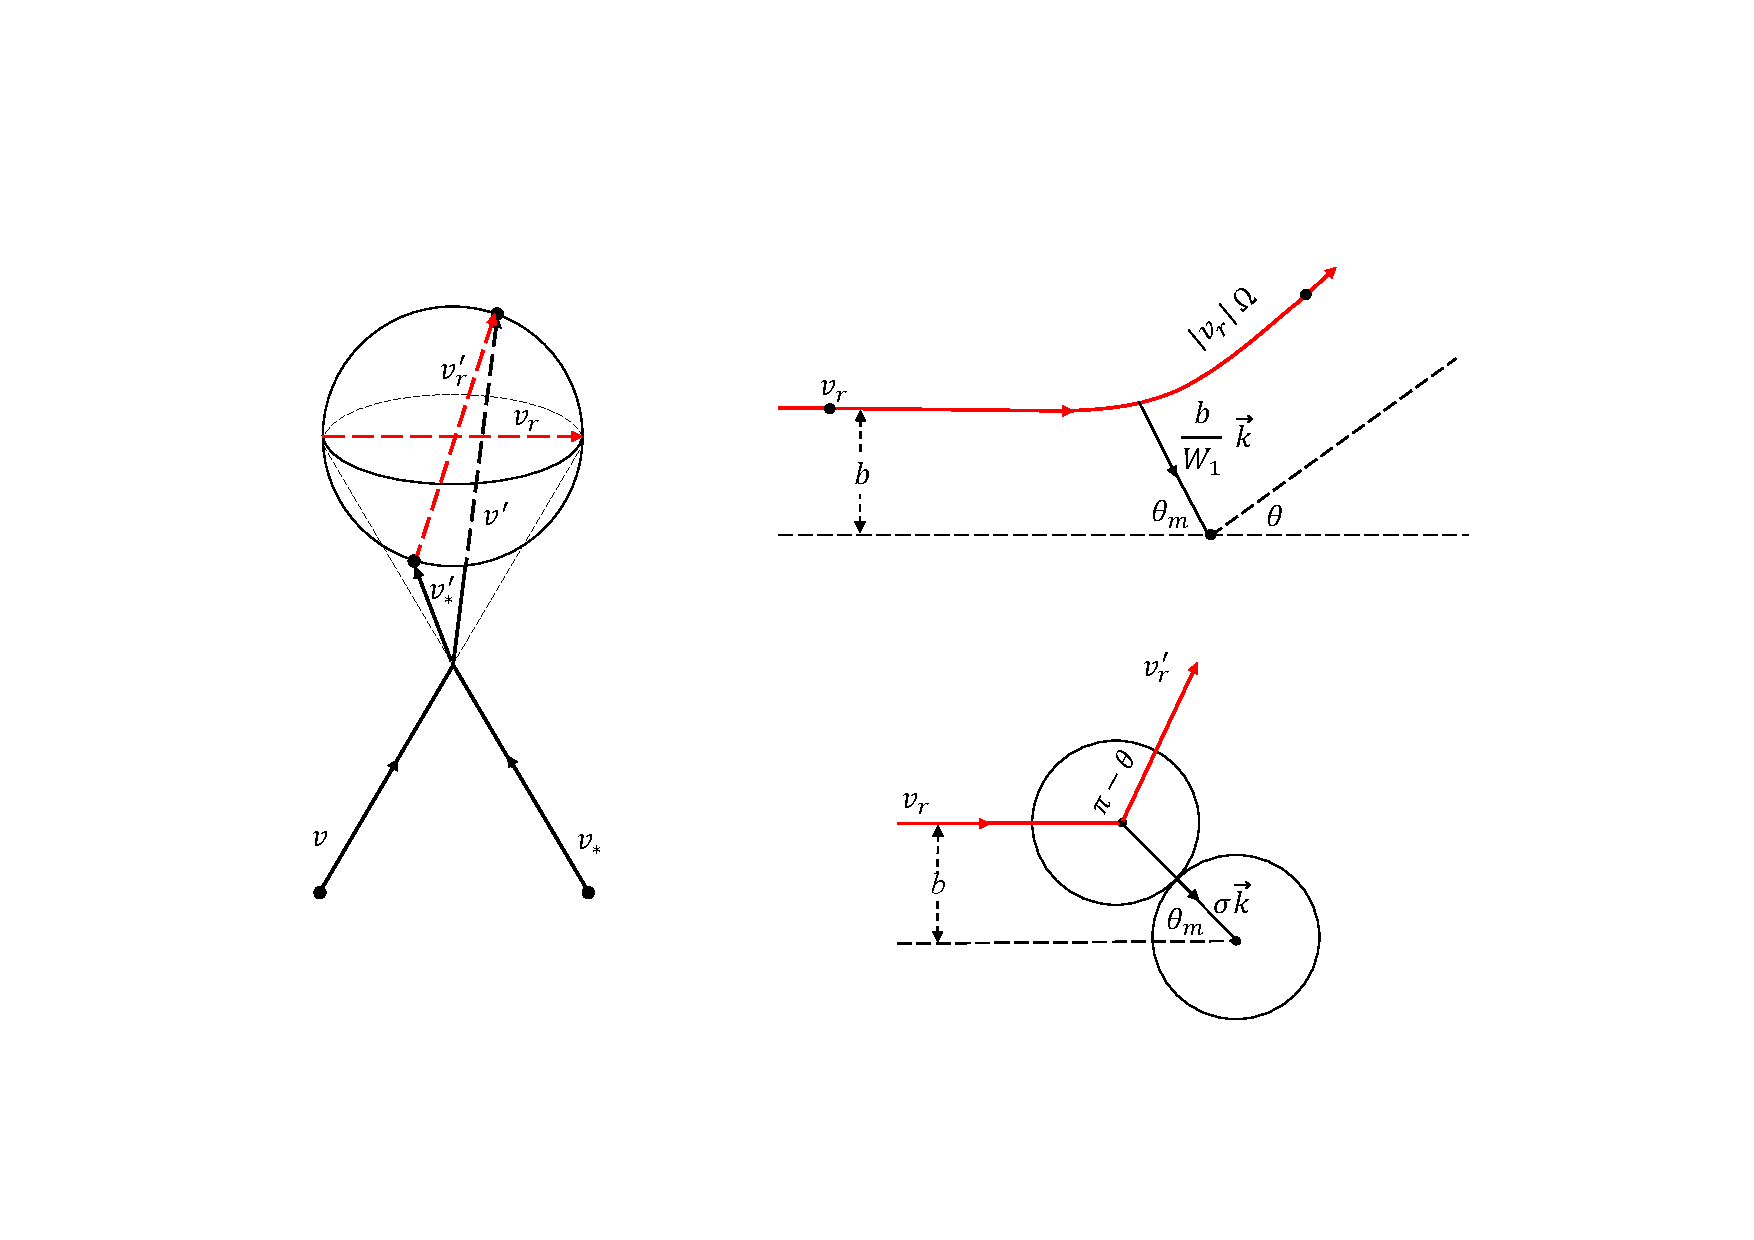
\includegraphics[width=0.9\textwidth]{Fig/Boltzmann_collision_demo.pdf}
	\caption{(左) 二体碰撞前后的速度分布. 由于动量和能量守恒,碰撞前后的相对速度分布在球体上并且通过球心.(右上)中心力场作用下的经典二体碰撞示意图,其中$b$ 为瞄准距离,$\bm{k}$ 为沿两分子间最短距离方向的单位矢量.(右下)直径为$\sigma$ 的硬球分子的两体碰撞.
	}
	\label{Boltzmann_collision_demo}
\end{figure}




\subsection{偏转角和微分散射截面}


假设分子间通过中心力场作用,作用势$\phi(r)$已知, 其中$r$为分子间距,则偏转角可以通过经典力学和量子力学两种方式求解.  若气体温度不低~(如氦气的温度高于100~K),两种方式得到的输运系数(如粘性和热导率)相同\cite{Sharipov2018Vacuum}. 这里仅介绍经典力学的计算结果,如图~\ref{Boltzmann_collision_demo}所示,偏转角可以表示为:
\begin{equation}\label{deflection}
\theta(b,{v}_r)=\pi-2\int_0^{W_1}\left[1-W^2-\frac{4\phi(r)}{m{v}_r^2}\right]^{-1/2}dW,
\end{equation}
其中,$W=b/r$为瞄准距离$b$与分子间距$r$的比值, 积分上限$W_1$对应于最短分子间距,即上式中括号内表达式等于零的方程的正根. 


%碰撞的微分散射截面为
%\begin{equation}\label{DCS_chapter1}
%\sigma_D=\frac{b|db|}{\sin\theta|d\theta|}=\left(\frac{m(\eta-1)}{4K}\right)^{2\eta-2}v^{-\frac{4}{\eta-1}}_r\times\frac{sds}{\sin\Theta{d\Theta}},
%\end{equation}
%碰撞核为
%\begin{equation}
%B(\theta,{v}_r)=v_r\sigma_D.
%\end{equation}


%although the Lennard-Jones potential is widely used (say, in the MD simulation of monatomic gas):
%\begin{equation}\label{Lennard_Jones_chapter}
%\phi(r_{ij})=4\epsilon\left[\left(\frac{d_{LJ}}{r_{ij}}\right)^{12}-\left(\frac{d_{LJ}}{r_{ij}}\right)^6\right],
%\end{equation}

%where $\epsilon$ is the potential depth and $d_{LJ}$ is the distance between two molecules where the potential is zero. 

在气体动理论中,经常考虑如下形式的逆幂律分子作用势:
\begin{equation}\label{power_law_potential}
\phi(r)=\frac{K}{\eta-1}r^{1-\eta},
\end{equation}
其中, $K$表征分子间相互作用的强度.  从公式~\eqref{deflection} 可知,偏转角只与变量$s$有关,即$\theta=\Theta(s)$:
\begin{equation}\label{impact_norm}
s=\left[\frac{m(\eta-1)}{4K}\right]^{\frac{1}{\eta-1}}bv^{\frac{2}{\eta-1}}_r.
\end{equation}

微分散射截面定义为
\begin{equation}\label{DCS_chapter1}
\begin{aligned}[b]
\sigma_D&=\frac{b|db|}{\sin\theta|d\theta|}\\
&=\left(\frac{m(\eta-1)}{4K}\right)^{\frac{2}{1-\eta}}v^{\frac{4}{1-\eta}}_r
\frac{sds}{\sin\Theta{d\Theta}},
\end{aligned}
\end{equation}
而碰撞核为
\begin{equation}
B(\theta,v_r)=v_r \sigma_D.
\end{equation}


当公式\eqref{power_law_potential}中$\eta=5$时,即为麦克斯韦分子,此时碰撞核与相对碰撞速度无关,记为 $B(\theta,v_r)=\sqrt{2K/m}B(\theta)$. 
对于硬球分子模型,可看作式\eqref{power_law_potential}中$\eta=\infty $,从图~\ref{Boltzmann_collision_demo}可以看出,偏转角可通过如下公式确定:
$b=\sigma\cos\left({\theta}/{2}\right)$,其中$\sigma$为硬球直径. 因此微分散射截面为 $\sigma_D={{\sigma}^2}/{4}$,而碰撞核为 $B(\theta,{v}_r)={\sigma}^2v_r/4$.  对于一般的气体,它们的行为介于麦克斯韦分子和硬球分子之间. 




\subsection{熵增原理}


对于任意关于分子速度的函数$\Psi(\bm{v})$,对玻尔兹曼碰撞项~\eqref{chapter1_collision} 在速度空间积分,具有如下对称性:
\begin{equation}\label{symmetry_collision}
\begin{aligned}[b]
\int\Psi(\bm{v})Q(\bm{v})d\bm{v}=&\frac{1}{4}\iiint d\Omega
d\bm{v}_\ast{d\bm{v}}
\Delta[\Psi]
B(\theta,v_r)\\
&\times \left[f(\bm{v}'_{\ast})f(\bm{v}')-f(\bm{v}_{\ast})f(\bm{v})\right],
\end{aligned}
\end{equation}
其中
$\Delta[\Psi]=
\Psi(\bm{v}_{\ast})+\Psi(\bm{v})
-\Psi(\bm{v}'_{\ast})-\Psi(\bm{v}')$. 
若$\Psi$满足 $\int\Psi(\bm{v})Qd\bm{v}=0$,则称其为碰撞不变量. 根据质量、动量和能量守恒,可知 $\Psi=1,\bm{v}, v^2$ 为碰撞不变量,而碰撞不变量的线性组合也是碰撞不变量. 

定义 $H$ 函数为:
\begin{equation}\label{entropy_function}
H=-\iint {f\ln}fd\bm{v}d\bm{x},
\end{equation}
是与气体系统的熵相关的标量.  在无外力的情况下,$H$ 的时间导数可写为:
\begin{equation*}
\begin{aligned}[b]
\frac{\partial H}{\partial t}=&	-\iint(1+{\ln}f)\frac{\partial{f}}{\partial{t}}d\bm{v}d\bm{x}\\
=&\iint{\bm{v}\cdot\frac{\partial{f}\ln{f}}{\partial\bm{x}}}d\bm{v}d\bm{x}-\iint(1+\ln{f}){Q} d\bm{v}d\bm{x}\\
=&\oint \int{\bm{v}\cdot\bm{n} {f}\ln{f}}d\bm{v}dS-\iint(1+\ln{f}){Q} d\bm{v}d\bm{x}.
\end{aligned}
\end{equation*}
式中,$\bm{n}$ 为系统表面微元 $dS$ 的外法线.  对于孤立系统,上式右端第一项为零;利用方程~\eqref{symmetry_collision},右端项第二项可写为:
\begin{equation*}
\begin{aligned}[b]
\frac{1}{4}\iiint{}&d\Omega
d\bm{v}_\ast{d\bm{v}}
B
\left[f(\bm{v}'_{\ast})f(\bm{v}')-f(\bm{v}_{\ast})f(\bm{v})\right]\\
&\times
\left\{
\ln[f(\bm{v}'_{\ast})f(\bm{v}')]
-\ln[f(\bm{v}_{\ast})f(\bm{v})]
\right\}.
\end{aligned}
\end{equation*}
因为碰撞核$B$非负,且对于任意的两个正整数 $a$ 和 $b$,不等式 $(a-b)(\ln{a}-\ln{b})\ge0$ 恒成立, 所以有
\begin{equation}\label{entropy_inequality}
\frac{\partial H}{\partial t}\ge0.
\end{equation}

上式表明孤立系统的$H$函数不会减小,这就是著名的玻尔兹曼的熵增原理. $H$随时间单调增加,但存在有限的上界,上界对应为式~\eqref{entropy_inequality}中等号成立时的平衡态, 即
$\ln{f}(\bm{v}_{\ast})+\ln{f}(\bm{v})
=\ln{f}(\bm{v}'_{\ast})+\ln{f}(\bm{v}')$. 
因此,$\ln{f}$ 也是碰撞不变量,可以表示为五个基本碰撞不变量 的线性组合:
$\ln{f}=\alpha_1+\bm{\alpha}_2\cdot\bm{v}+\alpha_3v^2$;给定系统的密度、速度和温度,
参数$\alpha_1$, $\alpha_3$ 和$\alpha_2$ 可以唯一确定. 此时,麦克斯韦平衡态速度分布函数为
\begin{equation}\label{equilibrium_Maxwellian}
F_{eq}(T)=n\left(\frac{m}{2\pi   k_BT}\right)^{3/2}\exp\left(-\frac{mc^2}{2k_BT}\right).
\end{equation}


\subsection{线性化玻尔兹曼方程}\label{LBE_chapter1}

线性化玻尔兹曼方程在气体动理论中具有重要地位. 第一,线性化玻尔兹曼碰撞项的本征值与本征函数,不仅在渐近展开推导纳维-斯托克斯方程的过程中至关重要,而且是发展简化动理学模型方程的源头理论. 第二,在许多微机电系统中,气体的压力梯度与温度梯度非常小,因此使用线性化方程可以高效准确地模拟微流动. 第三,虽然玻尔兹曼方程是单粒子速度分布函数确定性演化的平均方程,但是在某些问题中(例如:第\ref{RBS_section}节中的瑞利-布里渊散射)可以通过线化玻尔兹曼方程研究粒子涨落带来的影响. 

通常将速度分布函数在全局平衡态
\begin{equation}
f_{eq}=n_0\left(\frac{m}{2\pi   k_BT_0}\right)^{3/2}\exp\left(-\frac{mv^2}{2k_BT_0}\right)
\end{equation}
下展开为
\begin{equation}\label{chapter_vdf_lin_origin}
f(t,\bm{x},\bm{v})=f_{eq}(\bm{v})\left[1+\phi(t,\bm{x},\bm{v})\right],
\end{equation} 
其中扰动量 $\phi$ 满足约束条件 $|\phi|\ll1$. 不考虑外力项,只保留$\phi$的一次项,玻尔兹曼方程~\eqref{Boltzmann}可线性化为如下形式:
%\begin{widetext}
\begin{equation}\label{Chapter1_Boltzmann_lin0}
\begin{aligned}[b]
\frac{\partial\phi}{\partial t}+\bm{\xi}\cdot\frac{\partial\phi}{\partial
	\bm{x}}
&=\frac{\ell}{v_m}{J}(\phi)\\
&\equiv
-\frac{\ell}{v_m}\iint
B
\Delta[\phi]f_{eq}(\bm{v}_{\ast})d\Omega
d\bm{v}_\ast. %-\frac{2}{v_m}\bm{a}\cdot\bm{v}
\end{aligned}
\end{equation}
%\end{widetext}
这里的 速度 和 空间坐标分别通过最概然速率 $v_m$和特征尺寸 $\ell$ 进行无量纲化,时间用$\ell/v_m$归一化;无量纲分子速度为
\begin{equation}
\bm{\xi}=\frac{\bm{c}}{v_m(T_0)},
\end{equation}
其中
\begin{equation}
v_m(T)=\sqrt{\frac{2k_BT}{m}}
\end{equation}
为气体分子的最概然速率,即与麦克斯韦速率分布的极大值对应的速率. 

%\subsubsection{麦克斯韦气体:特征值和特征函数}
%\subsubsection{Maxwellian gas: eigenvalues and eigenfunctions}

对于麦克斯韦分子,线性化玻尔兹曼碰撞项的本征值与本征函数为~\cite{WangCS}:
\begin{equation}\label{Wang_Chang}
\begin{aligned}[b]
{J}(\Phi_{rlm})=&n\lambda_{rl}\Phi_{rlm},\\
\Phi_{rlm}=&g_{rl}(\xi)Y^m_{l}(\hat{\xi})
\\
=&\sqrt{\frac{2\pi^{3/2}r!}{\left(r+l+\frac{1}{2}\right)!}}
S^{(r)}_{l+\frac{1}{2}}(\xi^2)
\xi^l
Y^m_{l}(\hat{\xi}),\\
\lambda_{rl}=&2\pi\sqrt\frac{2K}{m}\int_0^\pi{}d\theta\sin\theta{B(\theta)}\\
&\times\left[-1+\cos^{2r+l}\frac{\theta}{2} 
P_l\left(\cos\frac{\theta}{2}\right) \right.\\
&\left. -\delta_{r0}\delta_{l0}+\sin^{2r+l}\frac{\theta}{2} 
P_l\left(\sin\frac{\theta}{2}\right)
\right].
\end{aligned} 
\end{equation}
式中,$P_l(x)$ 是勒让德多项式,$S^{(r)}_{l+\frac{1}{2}}(\xi)$ 是索南多项式,$Y^m_{l}(\hat{\xi})$ 为 $\bm{\xi}$方向的球谐函数. 


前三项本征值为 $\lambda_{00}=\lambda_{01}=\lambda_{10}=0$,分别代表三大守恒律. 另外两个非常重要的本征值为
\begin{equation}\label{eigenvalues}
\begin{aligned}[b]
\lambda_{02}=\left(-\frac{3}{2}\right)\pi\sqrt\frac{2K}{m}\int_0^\pi{d\theta}\sin^3\theta B(\theta), \\
\lambda_{11}=\frac{2}{3}\lambda_{02}, 
\end{aligned}
\end{equation}
它们决定剪切粘性系数和热导率的大小. 若归一化的速度$\bm{\xi}$在$z$轴的投影为$\xi_z=\xi\cos\theta$, 其中$\theta$为极距角,与上述本征值对应的本征函数为:
\begin{equation*}\label{eigenfunctions}
\begin{aligned}[b]
\Phi_{000}=1, ~
\Phi_{010}=\sqrt{2}\xi_z, ~
\Phi_{100}=\sqrt{\frac{2}{3}}\left(\frac{3}{2}-\xi^2\right), \\
\Phi_{020}=\frac{1}{3\sqrt{3}}\left(\xi^2_z-\frac{\xi^2}{3}\right),\\
\Phi_{110}=\frac{2}{\sqrt{5}}\left(\frac{5}{2}-\xi^2\right)\xi_z.
\end{aligned}
\end{equation*}
它们与气体的分子数密度、速度、温度、压力 和热流的扰动密切相关:
\begin{equation}\label{MP_KineticModel}
\begin{aligned}[b]
&[{n},\bm{u}, T]=\int\left[1,\bm{\xi},\frac{2}{3}\left(\xi^2-\frac{3}{2}\right)\right]
{f_{eq}\phi}d\bm{\xi}, \\
&[\sigma_{ij},\bm{q}]=\int
\left[2\xi_{\langle i}\xi_{j\rangle}, \left(\xi^2 -\frac{5}{2}\right)\bm{\xi}\right]
f_{eq}\phi{}d\bm{\xi}.
\end{aligned}
\end{equation}
其中,下标中出现尖括号表示该张量是无迹张量,即$\xi_{\langle i}\xi_{j\rangle}=\xi_i\xi_j-\xi^2\delta_{ij}/3$. 
为避免使用过多符号,在线性化问题中我们使用与原物理量相同的符号表示归一化的扰动物理量,如这里的扰动数密度$n$应理解为偏离参考数密度$n_0$的那部分,再除以参考数密度; 扰动温度$T$为偏离参考温度$T_0$的部分,再除以参考温度; 在全局平衡态下,参考速度、应力偏量和热流全部为零,因此上式中它们分别以$T_0$下的最概然速率$v_m$、$n_0k_BT_0$和 $n_0k_BT_0v_m$归一化. 

%;另外,我们默认在平衡态上进行扰动,因此参考速度、应力偏量和热流均为零
%\begin{equation}\label{MP_KineticModel}
%\begin{aligned}[b]
%{n}=\int{f_{eq}\phi}d\bm{v}, \\
%\bm{u}=\frac{1}{n_0}\int{\bm{v}f_{eq}\phi}d\bm{v}, \\
%T=\frac{2T_0}{3n_0}\int{\left(\frac{v^2}{v_m^2}-\frac{3}{2}\right)}
%f_{eq}\phi{}d\bm{v},  \\
%\sigma_{ij}=m\int
%v_{\langle i}v_{j\rangle}
%f_{eq}\phi{}d\bm{v}, \\
%\bm{q}=k_BT_0\int\left(\frac{v^2}{v_m^2} -\frac{5}{2}\right)\bm{v} f_{eq}\phi d\bm{v},
%\end{aligned}
%\end{equation}

\subsection{输运系数和弛豫率:表象与本质}

玻尔兹曼方程和纳维-斯托克斯方程分别在介观和宏观尺度上描述气体系统的演化,它们之间的关系一直是数学家和力学家研究的重要课题\cite{Sone2002Book}.  对玻尔兹曼方程求守恒量$m, m\bm{c},mc^2/2$的矩,可以得到如下宏观方程组:
\begin{equation}\label{macro}
\begin{aligned}[b]
\frac{\partial \rho}{\partial t}+\frac{\partial(\rho{}u_j) }{\partial x_j}=0, \\
\frac{\partial (\rho{u_i})}{\partial t}+\frac{\partial (\rho{}u_iu_j+p_{ij})}{\partial x_j}= \rho{}a_i,\\
\frac{\partial \left(\rho{}E\right)}{\partial t}+\frac{\partial \left(\rho{}{E}u_j+u_i{p}_{ij}+q_j\right)}{\partial x_j}=\rho{}a_ju_j,
\end{aligned}
\end{equation} 
其中$E=3k_BT/2m+u^2/{2}$. 但是该方程组并不封闭,因为压力张量和热流的表达式不能用密度、速度和温度表示.  有三种主要方法尝试封闭宏观方程组,它们分别是希尔伯特展开法\cite{Hilbert1912},Chapman-Enskog展开法~\cite{Chapman1916,enskog1917,CE}和矩方法\cite{Grad1949,henning}. 这里我们介绍最常用的第二种方法. 

在Chapman 和 Enskog~\cite{Chapman1916,enskog1917}方法中,首先将玻尔兹曼方程改写为:
\begin{equation}\label{expansion0}
\frac{\partial f}{\partial t}+\bm{v}\cdot\frac{\partial f}{\partial
	\bm{x}}+\bm{a}\cdot\frac{\partial f}{\partial \bm{v}}=\frac{Q(f)}{\epsilon}.
\end{equation} 
然后将分布函数和玻尔兹曼碰撞项展开为$\epsilon$ 的幂级数:
\begin{equation}\label{expansion1}
\begin{aligned}[b]
f=&\sum_{k=0}^\infty {\epsilon^k} f^{(k)},\\
Q=&\sum_{k=0}^\infty {\epsilon^k} Q^{(k)}=Q(f^{(0)})
+\epsilon{}{J}(f^{(1)})+O(\epsilon^2).
\end{aligned}
\end{equation}
值得注意的是,$\epsilon$是一个小的形式参数,主要用于监测展开的阶数. 展开完成后,取$\epsilon=1$. 

同时,压力和热流也相应展开如下:
\begin{equation}\label{shere_hilbert}
\begin{aligned}[b]
p_{ij} =\sum_{k=0}^\infty {\epsilon^k} p_{ij}^{(k)}
\equiv \sum_{k=0}^\infty {\epsilon^k} \times{}m\int{}c_ic_jf^{(k)}d\bm{v},
\\  
\bm{q} =\sum_{k=0}^\infty {\epsilon^k} \bm{q}^{(k)}
\equiv \sum_{k=0}^\infty {\epsilon^k} \times{}\frac{m}{2}\int{}\bm{c}c^2f^{(k)}d\bm{v}. 
\end{aligned}
\end{equation}
但是,碰撞不变量对应的宏观量 $C_M=\{\rho,\bm{u}, T\}$ 仅由分布函数的零阶展开决定,即
\begin{eqnarray}
[\rho,\rho\bm{u}, 3k_B\rho{}T]=m\int{}[1,\bm{v},mc^2]f^{(0)}d\bm{v}, \label{density_hilbert}
\end{eqnarray}
而各个高阶展开对$C_M$的贡献均为零,这称为兼容性条件. 


将公式~\eqref{shere_hilbert}代入公式~\eqref{macro},可知时间导数亦可表示为 $\epsilon$ 级数~\cite{henning}
\begin{equation}\label{fast_slow_time}
\frac{\partial}{\partial{} t}=\sum_{k=0}^\infty \epsilon^k \frac{\partial}{\partial{} t_k},
\end{equation}
且对于零阶近似,可得到
\begin{equation}\label{eq123_zerothOrder}
\begin{aligned}[b]
\frac{\partial \rho}{\partial t_0}+\frac{\partial(\rho{}u_j) }{\partial x_j}=0, \\
\frac{\partial (\rho{u_i})}{\partial t_0}+\frac{\partial (\rho{}u_iu_j+nk_BT\delta_{ij})}{\partial x_j}= \rho{}a_i,\\
\frac{\partial \left(\rho{}E\right)}{\partial t_0}+\frac{\partial \left(\rho{}{E}u_j+u_ink_BT\delta_{ij}\right)}{\partial x_j}=\rho{}a_ju_j.
\end{aligned}
\end{equation} 

从公式~\eqref{expansion0}和~\eqref{expansion1}易知$Q(f^{(0)})=0$. 因此,速度分布函数的零阶展开为
\begin{equation}
f^{(0)}=F_{eq}.
\end{equation} 
而速度分布函数的一阶近似$f^{(1)}=F_{eq}\phi$ 满足以下方程~\cite{henning}
%\begin{widetext}
\begin{equation}\label{integral_solution}
\begin{aligned}[b]
&{J}(\phi)=\frac{1}{F_{eq}}\left[\frac{\partial F_{eq}}{\partial t_0}+\bm{v}\cdot\frac{\partial F_{eq}}{\partial
	\bm{x}}+\bm{a}\cdot\frac{\partial F_{eq}}{\partial \bm{v}} \right]\\
&=
2\xi_{\langle{i}} \xi_{j\rangle}
\frac{\partial u_{\langle i}}{\partial x_{j\rangle}}
+\left(\xi^2-\frac{5}{2}\right)\xi_i\sqrt{\frac{2k_BT}{m}}\frac{\partial \ln{T}}{\partial x_i}.
\end{aligned}
\end{equation}
%\end{widetext}
其中,方程的推导过程中用到
\begin{equation*}
\frac{\partial F_{eq}}{\partial t_0}=
\frac{\partial F_{eq}}{\partial C_M}
\frac{\partial C_M}{\partial t_0}, \quad
\frac{\partial F_{eq}}{\partial \bm{x}}=
\frac{\partial F_{eq}}{\partial C_M}
\frac{\partial C_M}{\partial \bm{x}}, 
\end{equation*} 
以及公式~\eqref{eq123_zerothOrder}. 注意公式\eqref{Chapter1_Boltzmann_lin0}中的$f_{eq}$应改写为$F_{eq}$.


积分方程~\eqref{integral_solution}的解可分为齐次部分与非齐次部分,齐次部分满足 ${J}(\phi)=0$,这说明 $\phi$ 必然是碰撞不变量的线性组合,而兼容性条件要求所有线性组合的系数都为零. 非齐次部分满足如下形式
\begin{equation}
\phi=-A(\xi)\xi_i\sqrt{\frac{2k_BT}{m}}\frac{\partial \ln{T}}{\partial x_i}
-B(\xi)\xi_{\langle{i}} \xi_{j\rangle}\frac{\partial u_{\langle i}}{\partial x_{j\rangle}},
\end{equation}
其中,$A(\xi)$ 和 $B(\xi)$ 的解满足
\begin{equation}\label{transport_coefficient_0}
\begin{aligned}[b]
{J}(A\xi_i)&=-\left(\xi^2-\frac{5}{2}\right)\xi_i,
\\
{J}(B\xi_{\langle{i}} \xi_{j\rangle})&=-2\xi_{\langle{i}} \xi_{j\rangle},
\end{aligned}
\end{equation}
且兼容性条件要求$\int \xi^2A(\xi)F_{eq}d\bm{v}=0$. 


一旦得到$A(\xi)$ 和$B(\xi)$,通过一阶展开就可以恢复牛顿粘性定理与傅里叶热传导定理:
\begin{equation}\label{NS_constitutive}
\begin{aligned}[b]
\sigma^{(1)}_{ij}=-2\mu\frac{\partial u_{\langle i}}{\partial x_{j\rangle}},\quad
q^{(1)}_i=-\kappa \frac{\partial T}{\partial x_i},
\end{aligned}
\end{equation} 
且剪切粘性与热导率分别为
\begin{equation}\label{viscosity_original}
\begin{aligned}[b]
\mu=&\frac{2p}{15\pi^{3/2}}\int\exp(-\xi^2)B(\xi)\xi^4d\bm{\xi},
\\
\kappa=&\frac{2p}{3\pi^{3/2}}
\frac{k_B}{m}
\int\exp(-\xi^2)A(\xi)\xi^4
d\bm{\xi}.
\end{aligned}
\end{equation}


一般将$A(\xi)$ 和$B(\xi)$展开为索南多项式级数
\begin{equation}\label{sonine_expansion}
\begin{aligned}[b]
A(\xi)&=-\sum_{r=1}^{n_a}a_rS^{(r)}_{\frac{3}{2}}(\xi^2), \\
B(\xi)&=\sum_{r=0}^{n_b}b_rS^{(r)}_{\frac{5}{2}}(\xi^2),
\end{aligned}
\end{equation}
然后通过公式~\eqref{transport_coefficient_0}和索南多项式的正交性求解输运系数. 对于麦克斯韦分子,取第一项展开可得到准确的剪切粘性和热导率,即取$A(\xi)=a_1(\xi^2-5/2)$和$B(\xi)=b_0$;而对于其它相互作用势,仅考虑第一项展开得到的输运系数的相对误差也不超过2\%. 定义等效黏度截面为:
\begin{equation}
\sigma_{\mu}=\int \frac{B(\theta,v_r)}{v_r}\sin^2\theta {d\Omega},
%=2\pi\int_0^\pi \frac{B(\theta,v_m\eta)}{v_m\eta}\sin^3\theta {d\theta},
\end{equation}
则剪切粘性为
\begin{equation}\label{shear_CE_viscosity0}
\mu=\frac{5\sqrt{\pi{m}k_BT}}{8\left(\frac{m}{4k_BT}\right)^4\int_0^\infty
	{}v_r^7\sigma_{\mu}\exp\left(-\frac{mv^2_r}{4k_BT}\right)dv_r},
\end{equation}
而热导率为
\begin{equation}\label{shear_CE_thermal0}
{\kappa}=\frac{15}{4}\frac{k_B}{m}\mu,
\end{equation}
从而单原子气体的普朗特数为
\begin{equation}\label{Prandtl_number}
\begin{aligned}[b]
\Pr&={c_p}\frac{\mu}{\kappa}\\
&=\frac{5k_B}{2m}\frac{\mu}{\kappa}=\frac{2}{3}.
\end{aligned}
\end{equation}

对于逆幂律分子间相互作用势\eqref{power_law_potential},可以得出气体粘性和温度的关系
\begin{equation}\label{temperature_dependence}
\mu(T)\propto{T^\omega}, \quad
\omega=\frac{\eta+3}{2(\eta-1)},
\end{equation}
其中 $\omega$ 是粘性温度幂指数. 对于麦克斯韦分子和硬球分子,$\omega$ 分别取1和0.5; 对于其它气体,$\omega$一般介于0.5和1之间. 


%\leir{增大公式~\eqref{sonine_expansion}}中 $n_a$ 和 $n_b$ 的值,对结果的影响不大.例如,对于麦克斯韦分子,方程~\eqref{shear_CE_viscosity} 和方程~\eqref{shear_CE_thermal0} 是精确的,而对于硬球分子,当 $n_a=n_b=4$ 时,有
%%The results do not change much if we consider larger values of $n_a$ and $n_b$ in Eq.~\eqref{sonine_expansion}. For examples, for Maxwell molecules, Eqs.~\eqref{shear_CE_viscosity} and~\eqref{shear_CE_thermal0} are exact, while for HS molecules, if we consider $n_a=n_b=4$, we have
%\begin{equation}\label{transport_high_oder}
%\mu^{[4]}=1.016\mu^{[1]}, \\
%\kappa^{[4]}=1.025\kappa^{[1]}.
%\end{equation}
%对于幂指数在 $5\le\eta<\infty$ 范围内的逆幂律分子~\eqref{power_law_potential},修正因子介于麦克斯韦分子和硬球分子之间.

将公式~\eqref{NS_constitutive}代回公式~\eqref{macro}, 即可获得纳维-斯托克斯方程. 若继续计算Chapman-Enskog展开的高阶近似,可以得到Burnett、super-Burnett等宏观方程组\cite{CE}. 但是可能由于应力和热流与宏观量$C_M$展开的不匹配,导致高阶方程组的线性不稳定性. 同时,由于边界条件数量随着方程组阶数升高而增加,但对附加的边界条件提法缺少充分的研究,因此高阶方程组很少被实际应用. 另一方面,即使这些高阶方程组在某些情况下能得到精确解,解的精度也不一定随着展开阶数的增加而增加\cite{Gu2020AIA}. 

值得一提的是,对于麦克斯韦分子,在空间均匀系统中,本征值 $\lambda_{02}$ 和 $\lambda_{11}$ 与应力偏量和热流的弛豫速率相关,而这些弛豫速率决定着剪切粘性系数和热传导的大小:
\begin{equation}\label{universal_relation}
\begin{aligned}[b]
\frac{\partial \sigma_{ij}}{\partial t}
=&-n\lambda_{02} \sigma_{ij}=-\frac{p}{\mu}\sigma_{ij},\\
\frac{\partial q_{i}}{\partial t}=&-n\lambda_{11} q_{i}=-\frac{2}{3}\frac{p}{\mu}q_{i}.
\end{aligned}
\end{equation}
可以认为这些弛豫过程是本质,而粘性系数和热导率则为表象:在稀薄气体流动中,本构关系\eqref{NS_constitutive}和等效输运系数会随着克努森数的改变而改变,但一旦分子作用势确定,弛豫系数就会确定不变. 

利用弛豫时间和输运系数的关系,可以大大简化模型方程中输运系数的推导过程.  即,如果应力偏量的弛豫时间为$\tau$, 则剪切粘性为$p\tau$. 如果热流的弛豫时间为$\tau/A$,则普朗特数为$A$. 



% !TeX root = ../sustechthesis-example.tex

\chapter{图表示例}

\section{插图}

图片通常在 \env{figure} 环境中使用 \cs{includegraphics} 插入,如图~\ref{fig:example} 的源代码。
建议矢量图片使用 PDF 格式,比如数据可视化的绘图;
照片应使用 JPG 格式;
其他的栅格图应使用无损的 PNG 格式。
注意,LaTeX 不支持 TIFF 格式;EPS 格式已经过时。

\begin{figure}
  \centering
  \includegraphics[width=0.6\linewidth]{example-image-a.pdf}
  \caption{示例图片}
  \label{fig:example}
\end{figure}

若图或表中有附注,采用英文小写字母顺序编号,附注写在图或表的下方。
% LaTeX 传统上一般将附注的内容同图表的标题写在一起,形成很长的一段文字。

如果一个图由两个或两个以上分图组成时,各分图分别以(a)、(b)、(c)...... 作为图序,并须有分图题。
推荐使用 \pkg{subcaption} 宏包来处理, 比如图~\ref{fig:subfig-a} 和图~\ref{fig:subfig-b}。

\begin{figure}
  \centering
  \subcaptionbox{分图 A\label{fig:subfig-a}}
    {\includegraphics[width=0.45\linewidth]{example-image-a.pdf}}
  \subcaptionbox{分图 B\label{fig:subfig-b}}
    {\includegraphics[width=0.45\linewidth]{example-image-b.pdf}}
  \caption{多个分图的示例}
  \label{fig:multi-image}
\end{figure}



\section{表格}

表应具有自明性。为使表格简洁易读,尽可能采用三线表,如表~\ref{tab:three-line}。
三条线可以使用 \pkg{booktabs} 宏包提供的命令生成。

\begin{table}
  \centering
  \caption{三线表示例}
  \begin{tabular}{ll}
    \toprule
    文件名          & 描述                         \\
    \midrule
    thuthesis.dtx   & 模板的源文件,包括文档和注释 \\
    thuthesis.cls   & 模板文件                     \\
    thuthesis-*.bst & BibTeX 参考文献表样式文件    \\
    thuthesis-*.bbx & BibLaTeX 参考文献表样式文件  \\
    thuthesis-*.cbx & BibLaTeX 引用样式文件        \\
    \bottomrule
  \end{tabular}
  \label{tab:three-line}
\end{table}

表格如果有附注,尤其是需要在表格中进行标注时,可以使用 \pkg{threeparttable} 宏包。使用英文小写字母 a、b、c……顺序编号。

\begin{table}
  \centering
  \begin{threeparttable}[c]
    \caption{带附注的表格示例}
    \label{tab:three-part-table}
    \begin{tabular}{ll}
      \toprule
      文件名                 & 描述                         \\
      \midrule
      thuthesis.dtx\tnote{a} & 模板的源文件,包括文档和注释 \\
      thuthesis.cls\tnote{b} & 模板文件                     \\
      thuthesis-*.bst        & BibTeX 参考文献表样式文件    \\
      thuthesis-*.bbx        & BibLaTeX 参考文献表样式文件  \\
      thuthesis-*.cbx        & BibLaTeX 引用样式文件        \\
      \bottomrule
    \end{tabular}
    \begin{tablenotes}
      \item [a] 可以通过 xelatex 编译生成模板的使用说明文档;
        使用 xetex 编译 \file{thuthesis.ins} 时则会从 \file{.dtx} 中去除掉文档和注释,得到精简的 \file{.cls} 文件。
      \item [b] 更新模板时,一定要记得编译生成 \file{.cls} 文件,否则编译论文时载入的依然是旧版的模板。
    \end{tablenotes}
  \end{threeparttable}
\end{table}


如果您要排版的表格长度超过一页,那么推荐使用 \pkg{longtable} 或者 \pkg{supertabular}
宏包,模板对 \pkg{longtable} 进行了相应的设置,所以用起来可能简单一些。
表~\ref{tab:performance} 就是 \pkg{longtable} 的简单示例。

\begin{longtable}[c]{c*{6}{r}}
  \caption{实验数据(超长表格示例)}\label{tab:performance}\\
  \toprule[1.5pt]
   测试程序 & \multicolumn{1}{c}{正常运行} & \multicolumn{1}{c}{同步} & \multicolumn{1}{c}{检查点} & \multicolumn{1}{c}{卷回恢复}
  & \multicolumn{1}{c}{进程迁移} & \multicolumn{1}{c}{检查点} \\
  & \multicolumn{1}{c}{时间 (s)}& \multicolumn{1}{c}{时间 (s)}&
  \multicolumn{1}{c}{时间 (s)}& \multicolumn{1}{c}{时间 (s)}& \multicolumn{1}{c}{
    时间 (s)}&  文件(KB)\\\midrule[1pt]
  \endfirsthead
  \multicolumn{7}{c}{续表~\thetable\hskip1em 实验数据(超长表格示例)}\\
  \toprule[1.5pt]
   测试程序 & \multicolumn{1}{c}{正常运行} & \multicolumn{1}{c}{同步} & \multicolumn{1}{c}{检查点} & \multicolumn{1}{c}{卷回恢复}
  & \multicolumn{1}{c}{进程迁移} & \multicolumn{1}{c}{检查点} \\
  & \multicolumn{1}{c}{时间 (s)}& \multicolumn{1}{c}{时间 (s)}&
  \multicolumn{1}{c}{时间 (s)}& \multicolumn{1}{c}{时间 (s)}& \multicolumn{1}{c}{
    时间 (s)}&  文件(KB)\\\midrule[1pt]
  \endhead
  \bottomrule[1.5pt]
  \multicolumn{7}{r}{续下页}
  \endfoot
  \endlastfoot
  CG.A.2 & 23.05 & 0.002 & 0.116 & 0.035 & 0.589 & 32491 \\
  CG.A.4 & 15.06 & 0.003 & 0.067 & 0.021 & 0.351 & 18211 \\
  CG.A.8 & 13.38 & 0.004 & 0.072 & 0.023 & 0.210 & 9890 \\
  CG.B.2 & 867.45 & 0.002 & 0.864 & 0.232 & 3.256 & 228562 \\
  CG.B.4 & 501.61 & 0.003 & 0.438 & 0.136 & 2.075 & 123862 \\
  CG.B.8 & 384.65 & 0.004 & 0.457 & 0.108 & 1.235 & 63777 \\
  MG.A.2 & 112.27 & 0.002 & 0.846 & 0.237 & 3.930 & 236473 \\
  MG.A.4 & 59.84 & 0.003 & 0.442 & 0.128 & 2.070 & 123875 \\
  MG.A.8 & 31.38 & 0.003 & 0.476 & 0.114 & 1.041 & 60627 \\
  MG.B.2 & 526.28 & 0.002 & 0.821 & 0.238 & 4.176 & 236635 \\
  MG.B.4 & 280.11 & 0.003 & 0.432 & 0.130 & 1.706 & 123793 \\
  MG.B.8 & 148.29 & 0.003 & 0.442 & 0.116 & 0.893 & 60600 \\
  LU.A.2 & 2116.54 & 0.002 & 0.110 & 0.030 & 0.532 & 28754 \\
  LU.A.4 & 1102.50 & 0.002 & 0.069 & 0.017 & 0.255 & 14915 \\
  LU.A.8 & 574.47 & 0.003 & 0.067 & 0.016 & 0.192 & 8655 \\
  LU.B.2 & 9712.87 & 0.002 & 0.357 & 0.104 & 1.734 & 101975 \\
  LU.B.4 & 4757.80 & 0.003 & 0.190 & 0.056 & 0.808 & 53522 \\
  LU.B.8 & 2444.05 & 0.004 & 0.222 & 0.057 & 0.548 & 30134 \\
  EP.A.2 & 123.81 & 0.002 & 0.010 & 0.003 & 0.074 & 1834 \\
  EP.A.4 & 61.92 & 0.003 & 0.011 & 0.004 & 0.073 & 1743 \\
  EP.A.8 & 31.06 & 0.004 & 0.017 & 0.005 & 0.073 & 1661 \\
  EP.B.2 & 495.49 & 0.001 & 0.009 & 0.003 & 0.196 & 2011 \\
  EP.B.4 & 247.69 & 0.002 & 0.012 & 0.004 & 0.122 & 1663 \\
  EP.B.8 & 126.74 & 0.003 & 0.017 & 0.005 & 0.083 & 1656 \\
  EP.A.2 & 123.81 & 0.002 & 0.010 & 0.003 & 0.074 & 1834 \\
  EP.A.4 & 61.92 & 0.003 & 0.011 & 0.004 & 0.073 & 1743 \\
  EP.A.8 & 31.06 & 0.004 & 0.017 & 0.005 & 0.073 & 1661 \\
  EP.B.2 & 495.49 & 0.001 & 0.009 & 0.003 & 0.196 & 2011 \\
  EP.B.4 & 247.69 & 0.002 & 0.012 & 0.004 & 0.122 & 1663 \\
  EP.B.8 & 126.74 & 0.003 & 0.017 & 0.005 & 0.083 & 1656 \\
  EP.A.2 & 123.81 & 0.002 & 0.010 & 0.003 & 0.074 & 1834 \\
  EP.A.4 & 61.92 & 0.003 & 0.011 & 0.004 & 0.073 & 1743 \\
  EP.A.8 & 31.06 & 0.004 & 0.017 & 0.005 & 0.073 & 1661 \\
  EP.B.2 & 495.49 & 0.001 & 0.009 & 0.003 & 0.196 & 2011 \\
  EP.B.4 & 247.69 & 0.002 & 0.012 & 0.004 & 0.122 & 1663 \\
  EP.B.8 & 126.74 & 0.003 & 0.017 & 0.005 & 0.083 & 1656 \\
  EP.A.2 & 123.81 & 0.002 & 0.010 & 0.003 & 0.074 & 1834 \\
  EP.A.4 & 61.92 & 0.003 & 0.011 & 0.004 & 0.073 & 1743 \\
  EP.A.8 & 31.06 & 0.004 & 0.017 & 0.005 & 0.073 & 1661 \\
  EP.B.2 & 495.49 & 0.001 & 0.009 & 0.003 & 0.196 & 2011 \\
  EP.B.4 & 247.69 & 0.002 & 0.012 & 0.004 & 0.122 & 1663 \\
  EP.B.8 & 126.74 & 0.003 & 0.017 & 0.005 & 0.083 & 1656 \\
  \bottomrule[1.5pt]
\end{longtable}
% !TeX root = ../sustechthesis-example.tex

\chapter{数学符号和公式}

\section{数学符号}

研究生《写作指南》要求量及其单位所使用的符号应符合国家标准《国际单位制及其应用》(GB 3100—1993)、《有关量、单位和符号的一般原则》(GB/T 3101—1993)的规定。
模板中使用 \pkg{unicode-math} 宏包来配置数学符号,
与 \LaTeX{} 默认的英美国家的符号习惯有所差异:
\begin{enumerate}
  \item 大写希腊字母默认为斜体,如 \cs{Delta}:$\Delta$。
  \item 有限增量符号 $\increment$(U+2206)应使用 \pkg{unicode-math} 宏包提供的
    \cs{increment} 命令。
  \item 向量、矩阵和张量要求粗斜体,应该使用 \pkg{unicode-math} 的 \cs{symbf} 命令,
    如 \verb|\symbf{A}|、\verb|\symbf{\alpha}|。
  \item 数学常数和特殊函数要求用正体,应使用 \cs{symup} 命令,
    如 $\symup{\pi} = 3.14\dots$; $\symup{e} = 2.718\dots$,
  \item 微分号和积分号使用使用正体,比如 $\int f(x) \dif x$。
\end{enumerate}

关于数学符号更多的用法,参考
\href{http://mirrors.ctan.org/macros/latex/contrib/unicode-math/unicode-math.pdf}{\pkg{unicode-math}}
宏包的使用说明,
全部数学符号命的令参考
\href{http://mirrors.ctan.org/macros/latex/contrib/unicode-math/unimath-symbols.pdf}{\pkg{unimath-symbols}}。

关于量和单位推荐使用
\href{http://mirrors.ctan.org/macros/latex/contrib/siunitx/siunitx.pdf}{\pkg{siunitx}}
宏包,
可以方便地处理希腊字母以及数字与单位之间的空白,
比如:
\SI{6.4e6}{m},
\SI{9}{\micro\meter},
\si{kg.m.s^{-1}},
\SIrange{10}{20}{\degreeCelsius}。



\section{数学公式}

数学公式可以使用 \env{equation} 和 \env{equation*} 环境。
注意数学公式的引用应前后带括号,建议使用 \cs{eqref} 命令,比如式 \eqref{eq:example}。

\begin{definition}
  求余符号:“%”为求余符号。
\end{definition}

\begin{equation}
  \frac{1}{2 \symup{\pi} \symup{i}} \int_\gamma f = \sum_{k=1}^m n(\gamma; a_k) \mathscr{R}(f; a_k)
  \label{eq:example}
\end{equation}
注意公式编号的引用应含有圆括号,可以使用 \cs{eqref} 命令。

多行公式尽可能在“=”处对齐,推荐使用 \env{align} 环境。
\begin{align}
  a & = b + c + d + e \\
    & = f + g
\end{align}



\section{数学定理}

定理环境的格式可以使用 \pkg{amsthm} 或者 \pkg{ntheorem} 宏包配置。
用户在导言区载入这两者之一后,模板会自动配置 \env{thoerem}、\env{proof} 等环境。

\begin{theorem}[Lindeberg--Lévy 中心极限定理]
  设随机变量 $X_1, X_2, \dots, X_n$ 独立同分布, 且具有期望 $\mu$ 和有限的方差 $\sigma^2 \ne 0$,
  记 $\bar{X}_n = \frac{1}{n} \sum_{i+1}^n X_i$,则
  \begin{equation}
    \lim_{n \to \infty} P \left(\frac{\sqrt{n} \left( \bar{X}_n - \mu \right)}{\sigma} \le z \right) = \Phi(z),
  \end{equation}
  其中 $\Phi(z)$ 是标准正态分布的分布函数。
\end{theorem}
\begin{proof}
  Trivial.
\end{proof}

同时模板还提供了 \env{assumption}、\env{definition}、\env{proposition}、
\env{lemma}、\env{theorem}、\env{axiom}、\env{corollary}、\env{exercise}、
\env{example}、\env{remar}、\env{problem}、\env{conjecture} 这些相关的环境。

\section{数学字体}

\begin{equation}
  f(x)=a_0+ \sum_{n=1}^{\infty}   \left(  a_n\ \cos \frac{n\pi x}{L} +b_n  \sin⁡ \frac{n\pi x}{L}   \right)
\end{equation}

% !TeX root = ../sustechthesis-example.tex

\chapter{引用文献的标注}

模板支持以 BibTeX 的方式处理参考文献。
下文主要介绍 BibTeX 配合 \pkg{natbib} 宏包的主要使用方法。


\section{顺序编码制}

依学校样式规定,一般使用 \cs{cite},即序号置于方括号中,引文页码会放在括号外。统一处引用的连续序号会自动用短横线连接。

如多次引用同一文献,可能需要标注页码,例如:引用第二页\cite[2]{zhangkun1994},引用第五页\cite[5]{zhangkun1994}。

\thusetup{
  cite-style = super,
}
\begin{tabular}{l@{\quad$\Rightarrow$\quad}l}
  \verb|\cite{zhangkun1994}|               & \cite{zhangkun1994}   {\kaishu 不带页码的上标引用}            \\
  \verb|\cite[42]{zhangkun1994}|           & \cite[42]{zhangkun1994} {\kaishu 手动带页码的上标引用}          \\
  \verb|\cite{zhangkun1994,zhukezhen1973}| & \cite{zhangkun1994,zhukezhen1973}  {\kaishu 一次多篇文献的上标引用}  \\
\end{tabular}

注意,引文参考文献的每条都要在正文中标注
\cite{zhangkun1994,zhukezhen1973,dupont1974bone,zhengkaiqing1987,%
  jiangxizhou1980,jianduju1994,merkt1995rotational,mellinger1996laser,%
  bixon1996dynamics,mahui1995,carlson1981two,taylor1983scanning,%
  taylor1981study,shimizu1983laser,atkinson1982experimental,%
  kusch1975perturbations,guangxi1993,huosini1989guwu,wangfuzhi1865songlun,%
  zhaoyaodong1998xinshidai,biaozhunhua2002tushu,chubanzhuanye2004,%
  who1970factors,peebles2001probability,baishunong1998zhiwu,%
  weinstein1974pathogenic,hanjiren1985lun,dizhi1936dizhi,%
  tushuguan1957tushuguanxue,aaas1883science,fugang2000fengsha,%
  xiaoyu2001chubanye,oclc2000about,scitor2000project%
}。

引用测试:2个连续引用\cite{zhangkun1994,zhukezhen1973},2个间隔\cite{zhangkun1994,dupont1974bone},3个连续\cite{zhangkun1994,zhukezhen1973,dupont1974bone}。

\subsection{支持三级目录显示}

支持三级目录显示


\subsection{条目要求}

条目要求首行左缩进 2 个汉字符,避免悬挂缩进。如需使用带括号的条目列表,请自行添加 \verb|label=<style>| 参数。
下面是两个例子,还有更多用法,查阅 \pkg{enumitem} 宏包的文档。

默认条目序号:

\verb|\begin{enumerate} ... \end{enumerate}|

\begin{enumerate}
  \item 一级
  \begin{enumerate}
    \item 二级
    \begin{enumerate}
      \item 三级
      \begin{enumerate}
        \item 四级,《写作要求》未定义,请自行定义或者选择。
      \end{enumerate}
    \end{enumerate}
  \end{enumerate}
\end{enumerate}

自定义序号样式定义如表~\ref{tab:enum-style}。

\begin{table}[h]
  \centering
  \caption{条目样式选项}
  \label{tab:enum-style}
  \begin{tabular}{@{}ll@{}}
  \toprule
  \textbf{Code}          & \textbf{Description}                      \\ \midrule
  \textbackslash{}alph   & Lowercase letter (a, b, c, ...)           \\
  \textbackslash{}Alph   & Uppercase letter (A, B, C, ...)           \\
  \textbackslash{}arabic & Arabic number (1, 2, 3, ...)              \\
  \textbackslash{}roman  & Lowercase Roman numeral (i, ii, iii, ...) \\
  \textbackslash{}Roman  & Uppercase Roman numeral (I, II, III, ...) \\ \bottomrule
  \end{tabular}
\end{table}

\subsubsection{条目测试}


条目前文字,条目前文字,条目前文字,条目前文字,条目前文字,条目前文字,条目前文字,条目前文字,条目前文字,条目前文字,条目前文字。

\begin{enumerate}
  \item 一级条目,超长行。南方科技大学,南方科技大学,南方科技大学,南方科技大学,南方科技大学,南方科技大学,南方科技大学,南方科技大学,南方科技大学,南方科技大学,南方科技大学,南方科技大学,南方科技大学。
  \item 一级条目,南方科技大学,南方科技大学,南方科技大学。
  \item 一级条目,南方科技大学,南方科技大学,南方科技大学。
  \begin{enumerate}
    \item 二级条目,超长行。南方科技大学,南方科技大学,南方科技大学,南方科技大学,南方科技大学,南方科技大学,南方科技大学,南方科技大学,南方科技大学,南方科技大学,南方科技大学,南方科技大学,南方科技大学。
    \item 二级条目,南方科技大学,南方科技大学,南方科技大学。
    \item 二级条目,南方科技大学,南方科技大学,南方科技大学。
    \item 二级条目,南方科技大学,南方科技大学,南方科技大学。
    \item 二级条目,南方科技大学,南方科技大学,南方科技大学。
    \item 二级条目,南方科技大学,南方科技大学,南方科技大学。
    \begin{enumerate}
      \item 三级条目,南方科技大学,南方科技大学,南方科技大学。
      \item 三级条目,南方科技大学,南方科技大学,南方科技大学。
      \item 三级条目,南方科技大学,南方科技大学,南方科技大学。
      \begin{enumerate}
        \item \textbf{四级条目及之后的条目无规定序号格式,请自行设定选择。}
      \end{enumerate}
    \end{enumerate}
  \end{enumerate}
\end{enumerate}

条目后文字,条目后文字,条目后文字,条目后文字,条目后文字,条目后文字,条目后文字,条目后文字,条目后文字,条目后文字,条目后文字。

% !TeX root = ../sustechthesis-example.tex

\chapter{English Example}

If your supervisor is a foreign resident, or if your supervisor or defense committee specifically allows writing in English, the thesis may be written in English as the primary language. Please check with your supervisor or department secretary to confirm if you can write in English.

\section{Reference guide}

Writing in English still requires the Chinese reference standard GB/T 7714-2015.



% 结论
\backmatter
% !TeX root = ../sustechthesis-example.tex

\begin{conclusion}

学位论文的结论作为论文正文的最后一章单独排写,但不加章标题序号。

结论应是作者在学位论文研究过程中所取得的创新性成果的概要总结,不能与摘要混为一谈。博士学位论文结论应包括论文的主要结果、创新点、展望三部分,在结论中应概括论文的核心观点,明确、客观地指出本研究内容的创新性成果(含新见解、新观点、方法创新、技术创新、理论创新),并指出今后进一步在本研究方向进行研究工作的展望与设想。对所取得的创新性成果应注意从定性和定量两方面给出科学、准确的评价,分(1)、(2)、(3)…条列出,宜用“提出了”、“建立了”等词叙述。

\end{conclusion}



% 参考文献
\bibliography{ref/refs}  % 参考文献使用 BibTeX 编译
% \printbibliography       % 参考文献使用 BibLaTeX 编译,(不兼容本模板,请勿使用)

% 附录
\appendix
% !TeX root = ../sustechthesis-example.tex

\chapter{补充内容}

附录是与论文内容密切相关、但编入正文又影响整篇论文编排的条理和逻辑性的资料,例如某些重要的数据表格、计算程序、统计表等,是论文主体的补充内容,可根据需要设置。


\section{图表示例}

\subsection{图}

附录中的图片示例(图~\ref{fig:appendix-figure})。

\begin{figure}
  \centering
  \includegraphics[width=0.6\linewidth]{example-image-a.pdf}
  \caption{附录中的图片示例}
  \label{fig:appendix-figure}
\end{figure}


\subsection{表格}

附录中的表格示例(表~\ref{tab:appendix-table})。

\begin{table}
  \centering
  \caption{附录中的表格示例}
  \begin{tabular}{ll}
    \toprule
    文件名          & 描述                         \\
    \midrule
    sustechthesis.dtx   & 模板的源文件,包括文档和注释 \\
    sustechthesis.cls   & 模板文件                     \\
    thuthesis-*.bst & BibTeX 参考文献表样式文件    \\
    thuthesis-*.bbx & BibLaTeX 参考文献表样式文件  \\
    thuthesis-*.cbx & BibLaTeX 引用样式文件        \\
    \bottomrule
  \end{tabular}
  \label{tab:appendix-table}
\end{table}


\section{数学公式}

附录中的数学公式示例(公式\eqref{eq:appendix-equation})。
\begin{equation}
  \frac{1}{2 \uppi \symup{i}} \int_\gamma f = \sum_{k=1}^m n(\gamma; a_k) \mathscr{R}(f; a_k)
  \label{eq:appendix-equation}
\end{equation}


% 致谢
% !TeX root = ../sustechthesis-example.tex

\begin{acknowledgements}
  衷心感谢导师×××教授和物理系××副教授对本人的精心指导。他们的言传身教将使我终生受益。

  在美国麻省理工学院化学系进行九个月的合作研究期间,承蒙 Robert Field 教授热心指导与帮助,不胜感激。

  感谢×××××实验室主任×××教授,以及实验室全体老师和同窗们学的热情帮助和支持!

  本课题承蒙国家自然科学基金资助,特此致谢。
\end{acknowledgements}


% 个人简历、在学期间完成的相关学术成果
% !TeX root = ../sustechthesis-example.tex

\begin{resume}

  \section*{个人简历}
  % \section*{Resume}

  ××××年××月××日出生于××××。

  ××××年××月考入××大学××院(系)××专业,××××年××月本科毕业并获得××学学士学位。

  ××××年××月——××××年××月,在××大学××院(系)××学科学习并获得××学硕士学位。

  获奖情况:如获三好学生、优秀团干部、×奖学金等(不含科研学术获奖)。

  工作经历:……

  \section*{在学期间完成的相关学术成果}
  % \section*{Academic Achievements during the Study for an Academic Degree}

  “学术论文”和“申请及已获得的专利”使用 \env{localref} 环境生成,环境内使用 \cs{nocite}\{\texttt{<citekey>}\} 引用参考文献
  (与 \cs{cite}\{\texttt{<citekey>}\} 使用方式一致)。《指南》要求引用编号连续,故自行计算起始编号作为 \env{localref} 环境参数。“参与的科研项目及获奖情况”使用 \env{achievements} 环境生成,使用方式同 \env{enumerate} 环境,同样需要指定起始编号以满足《指南》要求。\textbf{本段在使用时请删除}。

  \subsection{学术论文}
  % \subsection{Academic papers}

  % \begin{localref}{参考文献路径}[起始序号(可选)]
  %   \nocite{引用条目代号} %% 使用方式同 \cite{}
  % \end{localref}

  \begin{localref}{ref/refs}
    \nocite{zhangkun1994}
    \nocite{bixon1996dynamics}
  \end{localref}


  \subsection{申请及已获得的专利(无获奖时此项不必列出)}
  % \subsection{Patents}

  % \begin{localref}{参考文献路径}[起始序号(可选)]
  %   \nocite{引用条目代号} %% 使用方式同 \cite{}
  % \end{localref}

  \begin{localref}{ref/refs}[3]
    \nocite{chenxu2020yejing}
    \nocite{jiangxizhou1980}
  \end{localref}

  \subsection{参与的科研项目及获奖情况(无获奖时此项不必列出)}
  \begin{achievements}[start=5]
    \item 姜锡洲,×××××研究,××省自然科学基金项目。课题编号:××××,长长长长长长长长长长长长长长长长长长长长长长长长长长长长长长长长长长长长长长长长长长长。
    \item ×××,×××××研究,××省自然科学基金项目。课题编号:××××。
    \item ×××,×××××研究,××省自然科学基金项目。课题编号:××××。
  \end{achievements}

\end{resume}


\end{document}
